% Ausarbeitung SAJ 
% FH Augsburg 
%
%
%
%
\documentclass[titlepage, 12pt,a4paper]{scrartcl}
%scrartcl
\usepackage[ngerman]{babel}
%\usepackage[latin1]{inputenc}
\usepackage[T1]{fontenc}
\usepackage{ucs}            % Eventuell benötigt
\usepackage[utf8x]{inputenc}

\usepackage{setspace}           % Paket fuer den Zeilenabstand
\onehalfspacing                 % Setzt den Zeilenabstand auf 1.5

\usepackage{graphicx}
\usepackage{listings}
\usepackage[hyphens]{url}
%\usepackage{breakurl}
\usepackage{hyperref}
\usepackage[usenames]{color}
\definecolor{light-gray}{gray}{0.90}
\usepackage[fixlanguage]{babelbib}
\usepackage{listings}
%\lstset{numbers=left, numberstyle=\tiny, numbersep=5pt}
%\lstset{language=Perl}
\lstloadlanguages{bash,XML,HTML, PHP, Python}
\selectbiblanguage{german}
\usepackage{makeidx}
%\usepackage{pifont}
\makeindex
%\usepackage{fancyhdr}
%\setlength{\headheight}{15.2pt}
%\pagestyle{fancy}


\author{Moritz Schächterle, Dominik Heimstädt \& Andrés Cuartas}
\title{- Studienarbeit Python - \\ WM-Tippspiel 2010 \\}
%\date{11-Dez-2007}

\pagestyle{myheadings}
\markright{Schaechterle, Heimstaedt \& Cuartas}
\lstset{
	inputencoding=utf8x,
	extendedchars=\true,
	language=Python,
	basicstyle=\tiny,
	keywordstyle=\bfseries\color{green},
	identifierstyle=,
	%commentstyle=\color{gray},	
	%stringstyle=\itshape\color{darkred},
	numbers=left,
	numberstyle=\tiny,
	stepnumber=1,
	breaklines=true,
	frame=none,
	showstringspaces=false,
	tabsize=4,
	backgroundcolor=\color{light-gray},
	captionpos=b,
	float=htbp,
	frameround=fttt
}


%\lstset{language=XML, stringstyle=\ttfamily, tabsize=2, basicstyle=\small, breaklines=true, backgroundcolor=\color{light-gray}, frameround=fttt}
%              
% WORKAROUND, damit lstlistoflistings funktioniert: 
% Quelle: http://www.komascript.de/node/477
%
\makeatletter% --> De-TeX-FAQ
\renewcommand*{\lstlistoflistings}{%
  \begingroup
    \if@twocolumn
      \@restonecoltrue\onecolumn
    \else
      \@restonecolfalse
    \fi
    \lol@heading
    \setlength{\parskip}{\z@}%
    \setlength{\parindent}{\z@}%
    \setlength{\parfillskip}{\z@ \@plus 1fil}%
    \@starttoc{lol}%
    \if@restonecol\twocolumn\fi
  \endgroup
}
\makeatother% --> \makeatletter 

\begin{document}

\maketitle
\newpage

\tableofcontents
\newpage

\section{Einführung}
Im Rahmen der Vorlesung „Internetprogrammierung mit Python“ ist eine
Studienarbeit zu erstellen. Aus mehreren zur Auswahl stehenden Arbeiten ist die
Wahl auf „Fußball-Tippspiel“ gefallen. Die Aufgabe darf im Team bearbeitet
werden mit maximal drei Gruppenmitgliedern. Aus aktuellem Anlaß wird die
Anwendug ein Fußball-WM Tippspiel mit der Möglichkeit auf die Begegnungen zu
tippen und für richtige Tipps, Differenz oder Tendenz Punkte zu erhalten. Die
Anwendung soll darüberhinaus noch ermöglichen einzusehen wieviele Punkte der
User momentan hat und auf welchen Platz er steht.

Bei der Überlegung zur Wahl geeigneter Werkzueuge zur Erstellung der Anwendung,
standen unter anderem Zope, Turbogears, Pylons und Django in der engeren
Auswahl.

Für die Auswahl geeigneter Werkzeuge sind folgende Punkte wichtig.
Arbeiten mit bekannten Techniken/Komponenten wie Python, mySQl,
ORM\footnote{Objekt-Relational Mapping}, HTML, JavaScript und Apache. 
Darüberhinaus sollte die Einarbeitungszeit nicht zu groß sein, da aus
Erfahrung, das Einarbeiten in neue Frameworks zeitaufwändig ist. Somit ist eine
gute Dokumentation ein weiterer wichtiger Punkt für die Auswahl.

Mit allen oben erwähnten Frameworks kommt man sicher schnell und einfach ans
Ziel. Letzenlich fiel die Wahl auf Django, da dieses Framework eine recht
schnelle Entwicklung für unsere Studienarbeit verspricht. Unter anderem sticht
die einfache Userverwaltung, der schnell zu konfigurierbare Adminbereich der
zur Verfügunggestellt wird, der OR-Mapper, das Templatesystem und der DRY: Don't
repeat yourself Ansatz. 

\section{Django}
Das Django Webframework eignet sich für die Erstellung von Webanwendungen. Es
folgt dem MVC\footnote{Model View Control} Muster. Wobei bei Django die Modelle
der Anwendung, die Objekte mit denen Django arbeitet mit Hilfe von OR-Mapping
in entweder mySQL, PostgreSQL, Oracle oder SQLite gespeichert werden können. So
wird die Datenpersistenz der Anwendung gewährleistet. Für die View sind
Templates zuständig, die mit Hilfe einer eigener Templatesprache konfiguriert
werden. Die Schnittstelle nach außen zum Server bieten die views (nicht zu
verwechseln mit der View), die die Kontrolle über die Anwendung bieten. Diese
beinhalten die Geschäftslogik und dienen als Verbindung zwischen den Modellen
und den Templates.


\section{Modelle}
\subsection{Klassen}
Für die Anwendung stand zuerst die Erstellung der Klassen bzw. der
Datenbankmodelle die benötigt werden, um die vorgestellten Ziele erreichen zu
können. Folgende Klassen werden für die Anwendung benötigt. 

\begin{figure}[ht]
 \begin{center}
  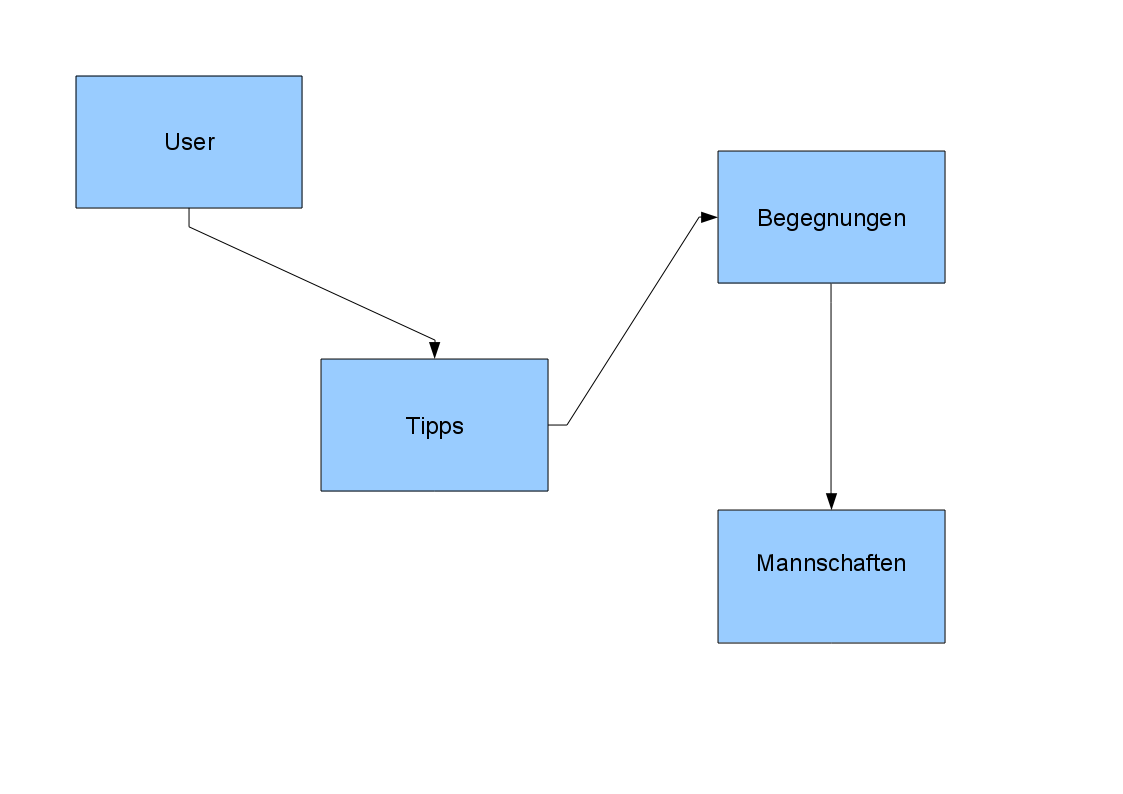
\includegraphics[scale=0.5]{pictures/klassen.png}
 \end{center}
 \caption{Benötigte Klassen}
 \label{klassen}
\end{figure}

Im Zentrum stehen die Tipps, welche die User abgeben können. Die Tipps setzen
sich zusammen aus den einzelnen Usern (Tipper) und den Spielbegegnungen. In
diesem Fall die Spiele der WM 2010. Weiterhin setzen sich diese aus Den
Mannschaften und weiteren Informationen, wie Spielzeit den Ergebnissen zusammen.
\\
\\

\begin{lstlisting}[caption=Modelle in Django]{modelleDjango}
class Tipps(models.Model):
    user = models.ForeignKey(User, unique=False)
    begegnung = models.ForeignKey(Begegnung, unique=False)
    
    toreHeim = models.IntegerField(max_length=2)
    toreGast = models.IntegerField(max_length=2)
    tippDatum = models.DateTimeField()
    
    def __unicode__(self):
        return u'%s %s' % (self.user, self.begegnung)
   
\end{lstlisting}

\subsection{OR-Mapping}
Mit Hilfe des eingebauten OR-Mappers in Django können die Tabellen aus den
vorher definierten Klassen als Tabellen in die Datenbank gespeichert werden.
Die Speicherung bzw. Synchronisation geschieht mit Django eigenen Boardmitteln.

\begin{lstlisting}[caption=Datenbanksynchronisation]{sync}
python manage.py syncdb
\end{lstlisting}

Damit Python mit der Datenbank kommunizieren kann muss vorher ein
Datenbank-Connector installiert werden. Django unterstützt Oracle, PostgreSQL,
MySQL und SQLite. Die Installation des Connectors ist abhängig von der
Datenbank, die benutzt werden soll. Getestet wurden mySQL und PostgreSQL
hierbei bei der lokalen Entwicklung unter Ubuntu mySQL und auf dem
Produktionsserver Postgres. Bei der Speicherung und Auslesen der Daten erwies
sich mySQL toleranter, für den Produktionsserver mussten drei
Views\footnote{Django funktion} für PostgreSQL angepasst werden, weil
Exceptions von Django zurückgegeben wurden, die auf Probleme mit dem Speichern
und Auslesen von Daten zurückzuführen waren.

\subsection{Administration}
Mit Hilfe der Django eigenen Administrationsoberfläche, die einfach als
Applikation in der \emph{settings.py}\footnote{Datei beinhaltet alle
Umgebungsvariablen des Projektes} installiert werden kann, können leicht die
benötigten Einträge in die Datenbank geschrieben werden. Auch
\emph{Datetime-Felder} werden erkannt und es werden spezielle Widgets für die
Eintragung von Datenfeldern zur Verfügung gestellt. In dem Zusammenhang wurde
entschienden, die benötigten Informationen über Skripte, automatisch befüllen zu
lassen genaueres im Kapitel \ref{hilfsskripte} auf Seite \pageref{hilfsskripte}. 


\section{Views}
\subsection{Funktionalität}
Die Geschäftslogik wird mit Hilfe der Views erstellt. Der Name ist hier etwas
irreführend, weil man View mit der Ausgabe, also HTML verküpft. Die View ist die
Schnittstelle, mit der die Anwendung mit dem Server/Client kommuniziert. Im
wmTippspiel wird beim Aufruf der Startseite, automatisch die dafür zuständige
View angesprochen. Diese führt Befehle aus, die ihre Ergenisse einem Template
übergeben kann. Das Template generiert aus den übergebenen Informationen
schließlich dann HTML, welches dem Server zur Weiterleitung an den Client zur
Verfügung gestellt wird.

\subsection{URL-Dispatching}
In Django gibt es eine Kontrollinstanz, die ermöglicht, abhängig von der URL,
auf die verschiedenen Views der Seite zu verweisen. Einstellungen können in der
\emph{urls.py} gemacht werden. Mit Hilfe regulärer Audrücke wird die URL
untersucht. Der erste Ausdruck auf dem die URL passt, ermittelt und
die dahinterliegende View ausgeführt.

\begin{lstlisting}[caption=Auszug ursl.py]{urls.py}
urlpatterns = patterns('',
    (r'^$', index ),
    (r'^time/$', current_datetime ),
    (r'^displaymeta/$', display_meta ),
    #(r'^login/$', mylogin ),
    (r'^accounts/logout/$', 'django.contrib.auth.views.logout', {'next_page':'/'}),
    (r'^accounts/login/$', 'django.contrib.auth.views.login'),
    # Example:
    # (r'^wmTippspiel/', include('wmTippspiel.foo.urls')),

    # Uncomment the admin/doc line below and add 'django.contrib.admindocs'
    # to INSTALLED_APPS to enable admin documentation:
    # (r'^admin/doc/', include('django.contrib.admindocs.urls')),

    # Uncomment the next line to enable the admin:
    (r'^admin/', include(admin.site.urls)),
    
    (r'^tippspiel/', include('wmTippspiel.appWMTippspiel.urls')),
    
)
\end{lstlisting}

\subsection{Django App}
Im wmTippspiel wurde eine App\footnote{Eigenständiger Teil einer Webanwendung,
kann in verschiedenen Projekten eingebunden werden} erstellt und ausgelagert, so
kann die erstellte Applikation auch in anderen Internetseiten ohne viel Aufwand 
eingbunden werden.

\begin{lstlisting}
(r'^tippspiel/', include('wmTippspiel.appWMTippspiel.urls')),
\end{lstlisting}

Die appWMTippspiel bildet den Kern des wmTippspiel-Projekts. Daneben sind
weitere Applikationen, wie eine Registrierungs-Applikation
(siehe Kapitel \ref{registrierung}) denkbar, damit sich User bequem auf der
Seite registrieren können. Diese Applikation kann thematisch gut von der 
appWMTippspiel abgegrenzt werden und in anderen Projekten eingesetzt werden. 
Was zu dem Don't repeat Yourself Gedankten Djangos passt.

\section{Login und Registrierung}\label{registrierung}
\subsection{User-Authentifikation}
In unserem Projekt stellte sich das User-Authentifikation-System als eines der
drei größeren UseCases heraus. Wichtig erschien uns, dass der Besucher beim 
ersten Besuch ohne großen Zeitaufwand einen Account erstellen kann und dann 
gleich mit Tippen loslegen kann, also eine Registrierung mit automatischem 
Login. Später, bei jedem weiteren Besuch, erfolgt dann der gewohnte Login per 
Username und Passwort. Da die Registrierung, auch aufgrund unseres Layouts, 
nicht mit einem zweiten Passwortkontrollfeld ausgestattet ist, musste
zusätzlich noch eine „Passwort vergessen?“-Funktionalität eingebaut werden.

Die Arbeit mit dem Web-Framework Django ermöglichte nun den Einsatz des 
Framework eigenen Authentifizierung-Werkzeuges, zu dem hier zunächst ein
kleiner Einblick zu der Arbeitsweise gegeben werden soll. Django setzt dabei
auf eine User-Session mit Cookie zur Speicherung der Session-ID, ein Verfahren,
das mittlerweile bei so ziemlich jedem Framework oder CMS Standard ist. Als 
Aufgabenfelder dienen die Verwaltung von User, Gruppen und deren
Berechtigungen. Da wir in unserem Projekt nur die Gruppierungen der normalen 
User und Superuser (nur für auto-generierten Admin-Bereich) benutzen und selbst
keine eigenen Gruppen anlegen, wird hier nur das User-Model vorgestellt. Im
Grunde genommen benötigen wir für dieses nur die User-Daten Username, Passwort,
Emailadresse und ein paar versteckte Daten, wie „is\_active“, „last\_login“,
etc. So gesehen, reicht uns also das Django eigene User-Model völlig aus und 
kann gleich so übernommen werden. Auch bei den Berechtigungen kommen wir relativ 
spartanisch zurecht, weil wir nur zwischen Inhalten unterscheiden, die der 
eingeloggte User sehen darf und solche, die jeder Besucher sehen darf 
(Admin-Bereich ist außen vor!). Hier reicht also auch nur eine einfache
Prüfung,  welche Django selbst in der View-Datei per „Shortcut“ übernimmt:

\begin{lstlisting}[caption=Hibernate]{Login decorator}
@login_required
    def meinView(request):
    bspVar = 1 …
\end{lstlisting}

\subsection{Admin-Bereich für das User-Management}
Zuallererst eine gute Nachricht: das Entwickeln des Admin-Bereichs  (eine
aufwendige Aufgabe, deren Mühen der normale Besucher nicht würdigt) kann man 
sich mit Django getrost sparen. Es generiert automatisch für jedes erstellte 
Model gewünschte Formulare in einem geschützten Admin-Bereich, der nur für die 
oben angesprochenen Superuser zugänglich ist. Einzelne Änderungen der Formulare
oder Bedienbarkeit können mit Hilfe der Django Online-Dokumentation schnell 
gemacht werden, meistens sind sie aber nicht von Nöten.


\subsection{Login-Werkzeug von Django}
Auch beim Erstellen eines Logins kann man sich im Großen und Ganzen auf die 
Bibliothek django.contrib.auth.views.login verlassen.. Dies kann ganz einfach 
direkt in der url.py aufgerufen werden, wahlweise mit einem Template oder auch 
ganz spartanisch ohne. Hat man sich für ein Template entschieden, ist es hier 
möglich sich die Input-Felder (HTML) per Django's eigener Template-Sprache 
generieren zu lassen, oder, wie wir es gemacht haben, selbst mit HTML zu 
erstellen. Dies ermöglichte uns einen schnelleren Zugriff auf die Attribute des
Input-Feldes, da wir Änderungen aus layouttechnischen Gründen benötigten. Ein 
interessantes Feature bietet die „next“-Funktion des Logins, die als 
GET-Parameter übergeben, dem Besucher besseres Navigieren erlaubt: z.B. möchte 
der nicht eingeloggte User in der Galerie ein Bild betrachten. Dies ist jedoch 
nur authentifizierten Usern gestattet. Deshalb wird ein next-Parameter 
mitgegeben, in welchem die Adresse zu dem Bild gespeichert wird, damit er nach 
erfolgreichem Login dort auch landet.


\subsection{Logout bei Django}
Für den Logout reicht ebenfalls die vorgegeben Funktion 
django.contrib.auth.views.logout in der urls.py einzustellen, da sie ja kein 
eigenes Template oder besondere Einstellungen bedarf.


\subsection{Registrierung}
Für die Registrierung selbst gibt es allerdings keine Hilfen seitens Django, da
sie meist eine sehr individuelle Sache ist, z.B. möchte man bei einer Webshop 
Kontodaten, bei einer Online-Community vielleicht Geburtsdatum und Hobbies usw.
wissen. Auch bieten sich hier besondere Sicherungsmöglichkeiten wie Captcha
etc.  an, was wir allerdings für unser kleines Tippspiel aufgrund der geringen 
Laufzeit nicht benötigten. Da wir einen schnellen Einstieg für den Teilnehmer 
uns wünschten, verzichteten wir außerdem auf eine Aktivierungsemail und loggten
den User sofort nach der Registrierung ein.

\subsection{Passwort vergessen}
Da eine erleichterte Registrierung schnell zu fehlerhaften bzw. vergessenen 
Passwörtern führen kann, wurde noch eine „Passwort vergessen“-Funktion 
eingeführt, die dem Teilnehmer nach dem Eintragen seiner E-mailadresse, sein 
neues, zufallsgenerierte Passwort zuschickt. Bei der Entwicklung dieser
Funktion  kann man sich auch hier wieder auf Django verlassen, das ein Werkzeug
zum E-mail versenden anbietet, als auch eine Funktion zur Erstellung von 
zufälligen Passwörtern, was jedoch bei uns selbst durch ein kleinen Einzeiler 
programmiert wurde.

\section{Hilfsskripte}\label{hilfsskripte}

\section{Templates}
\section{Portierung auf Produktionsserver}
\section{Fazit}


\end{document}
